\documentclass[tikz,border=5mm]{standalone}

\usepackage{tikz}
\usetikzlibrary{calc,arrows.meta}

\newcommand{\Xc}{\mathcal{X}}

\begin{document}

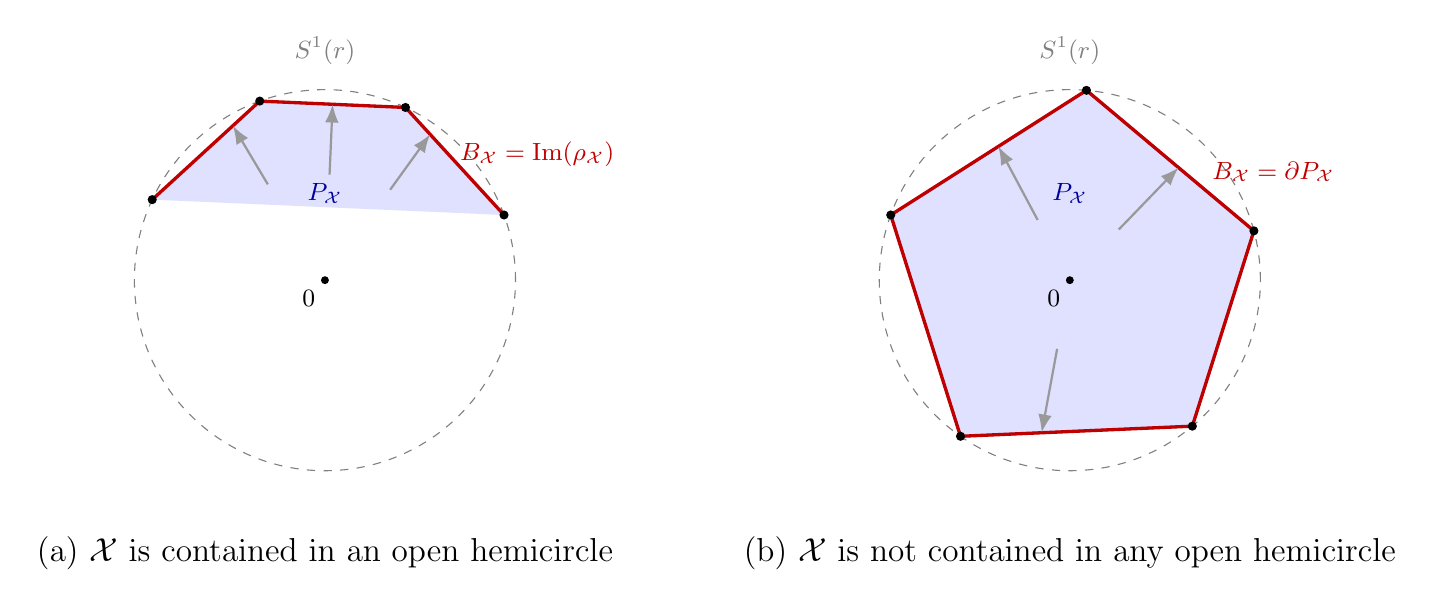
\begin{tikzpicture}[scale=1.1,>=Latex,font=\small]
    \def\r{2.2}
    \def\shift{4.3} % half of the distance between the two centers

    %======================================================
    % (a) X contained in an open hemicircle
    %======================================================
    \begin{scope}[xshift=-\shift cm]
        \coordinate (O) at (0,0);

        % circle S^1(r)
        \draw[dashed,gray] (O) circle (\r);
        \node[gray] at (0,2.65) {$S^1(r)$};

        % points of X
        \coordinate (A1) at (20:\r);
        \coordinate (B1) at (65:\r);
        \coordinate (C1) at (110:\r);
        \coordinate (D1) at (155:\r);

        % convex hull P_X
        \fill[blue!12] (A1)--(B1)--(C1)--(D1)--cycle;
        \node[blue!60!black] at (0,1.0) {$P_{\Xc}$};

        % image of rho
        \draw[very thick,red!75!black] (A1)--(B1)--(C1)--(D1);
        \node[red!75!black,align=center] at (2.45,1.45)
            {$B_{\Xc}=\mathrm{Im}(\rho_{\Xc})$};

        % sample arrows
        \coordinate (T11) at ($(A1)!0.35!(B1)$);
        \coordinate (T12) at ($(A1)!0.75!(B1)$);
        \coordinate (T13) at ($(B1)!0.50!(C1)$);
        \coordinate (T14) at ($(C1)!0.25!(D1)$);
        \coordinate (T15) at ($(C1)!0.70!(D1)$);

        \coordinate (S11) at ($(O)!0.65!(T11)$);
        \coordinate (S12) at ($(O)!0.62!(T12)$);
        \coordinate (S13) at ($(O)!0.60!(T13)$);
        \coordinate (S14) at ($(O)!0.62!(T14)$);
        \coordinate (S15) at ($(O)!0.65!(T15)$);

        % \draw[->,gray!80,thick] (S11)--(T11);
        \draw[->,gray!80,thick] (S12)--(T12);
        \draw[->,gray!80,thick] (S13)--(T13);
        \draw[->,gray!80,thick] (S14)--(T14);
        % \draw[->,gray!80,thick] (S15)--(T15);

        % points
        \foreach \P in {A1,B1,C1,D1}{
            \fill (\P) circle (1.5pt);
        }

        % origin
        \fill (O) circle (1.3pt);
        \node[below left] at (O) {$0$};

        \node[font=\large] at (0,-3.15)
            {(a) $\Xc$ is contained in an open hemicircle};
    \end{scope}

    %======================================================
    % (b) X not contained in any open hemicircle
    %======================================================
    \begin{scope}[xshift=\shift cm]
        \coordinate (O) at (0,0);

        % circle S^1(r)
        \draw[dashed,gray] (O) circle (\r);
        \node[gray] at (0,2.65) {$S^1(r)$};

        % points of X
        \coordinate (A2) at (15:\r);
        \coordinate (B2) at (85:\r);
        \coordinate (C2) at (160:\r);
        \coordinate (D2) at (235:\r);
        \coordinate (E2) at (310:\r);

        % convex hull P_X
        \fill[blue!12] (A2)--(B2)--(C2)--(D2)--(E2)--cycle;
        \draw[thick,blue!60!black] (A2)--(B2)--(C2)--(D2)--(E2)--cycle;
        \node[blue!60!black] at (0,1.0) {$P_{\Xc}$};

        % image of rho
        \draw[very thick,red!75!black] (A2)--(B2)--(C2)--(D2)--(E2)--cycle;
        \node[red!75!black,align=center] at (2.35,1.25)
            {$B_{\Xc}=\partial P_{\Xc}$};

        % sample arrows
        \coordinate (T21) at ($(A2)!0.45!(B2)$);
        \coordinate (T22) at ($(B2)!0.45!(C2)$);
        \coordinate (T23) at ($(D2)!0.35!(E2)$);

        \coordinate (S21) at ($(O)!0.45!(T21)$);
        \coordinate (S22) at ($(O)!0.45!(T22)$);
        \coordinate (S23) at ($(O)!0.45!(T23)$);

        \draw[->,gray!80,thick] (S21)--(T21);
        \draw[->,gray!80,thick] (S22)--(T22);
        \draw[->,gray!80,thick] (S23)--(T23);

        % points
        \foreach \P in {A2,B2,C2,D2,E2}{
            \fill (\P) circle (1.5pt);
        }

        % origin
        \fill (O) circle (1.3pt);
        \node[below left] at (O) {$0$};

        \node[font=\large] at (0,-3.15)
            {(b) $\Xc$ is not contained in any open hemicircle};
    \end{scope}
\end{tikzpicture}

\end{document}